\documentclass[oneside,openany]{book}

  \usepackage{color}
  \usepackage{booktabs}
  \usepackage{placeins}
  \usepackage{mdframed}
  \usepackage{titlesec}
  \usepackage{float}
  \usepackage{fancyhdr}
  \usepackage{xcolor}
  \usepackage[bookmarks=true,bookmarksnumbered=true,bookmarksopen=true,pdftex,pdfstartview=FitH]{hyperref}
  \usepackage{xeCJK}
  %\setCJKmainfont{SimSun}
  \setCJKmainfont[BoldFont={SimHei}]{SimSun}

  \title{Vim-Sztools使用手册}
  \author{左晃右过<shrek.wang挨特gmail.com>}

  \setlength{\parskip}{0.5em}
  \restylefloat{table}
  \restylefloat{figure}
  \pagestyle{fancy}
  \titleformat{\chapter}{\centering\Huge\bfseries}{第\,\thechapter\,章}{1em}{}

  \mdfdefinestyle{BestPracticeFrame}{
    linecolor=black,
    topline=false,
    rightline=false,
    leftline=false,
    bottomline=false,
    outerlinewidth=0pt,
    roundcorner=20pt,
    innertopmargin=\baselineskip,
    innerbottommargin=\baselineskip,
    innerrightmargin=10pt,
    innerleftmargin=10pt,
    backgroundcolor=gray!50!white}

  \mdfdefinestyle{SmallFrame}{
    linecolor=black,
    topline=false,
    rightline=false,
    leftline=false,
    bottomline=false,
    outerlinewidth=0pt,
    roundcorner=5pt,
    innertopmargin=5pt,
    innerbottommargin=5pt,
    innerrightmargin=3pt,
    innerleftmargin=3pt,
    backgroundcolor=gray!50!white}

\begin{document}
\maketitle

\chapter{简介}

  \begin{center}
    \large\textbf{工欲善其事,必先利其器}
  \end{center}

  对于开发人员来说,选好一个工具并用到纯熟,无疑对工作效率有很好的提升。 文本编辑器,编译器,调试
器就是开发必不可少的几个工具。  Vim是功能最强大的文本编辑器之一(另一个是Emacs)。 
但是Vim中可选的java开发类插件并不多, 可能是用Vim做java开发的程序员太少了。 许多Java程序员现在都用的是eclipse,jbuilder之类
的IDE, 不过eclipse除了其臭名昭著的体积庞大,运行慢等缺点之外, 其编辑功能跟vim比起来,实在连鸡肋都算不上。 

  vim的java开发插件虽不多,但是在vim官网已经有一个比较著名的java开发插件,VJDE。 另外eclim直接
将eclipse做为后端, 将很多功能直接引入了vim。 而eclipse本身作为一个开发工具平台,上面也有形形色色的仿
vim插件(参见附录)。因此无论是在vim中用java开发类插件或是在eclipse中安装vim插件启用vim模式, 似乎都有不错的选择。
为什么还要再做一个插件Vim-Sztool呢
  
  \begin{enumerate}
    \item VJDE每次补全都需调用外部java命令用反射来读取类信息,速度比较慢。eclim因为用eclipse作为后端, 速度也是偏慢。
    \item 无法在vim中调试java程序。
    \item 此处省略n条理由...
  \end{enumerate}

  相比于现有的java开发类插件,Vim-Sztool有自己的一些特色
  \begin{enumerate}
    \item 快速的补全(类相关信息缓存在Agent中)
    \item java程序调试功能,可能是仅有的支持java调试的vim插件
    \item 定制的ProjectTree,项目中引用的源码包(source jar)也按树结点显示。
    \item 快速文件定位,类似于Eclipse中的open resource功能。
    \item 源码跳转,支持跳转到source jar包中的文件。
    \item 自带jdb支持java程序调试并支持远程调试
    \item 直接从自带jdb中启动tomcat
  \end{enumerate}

  Vim-Sztool采用了类似eclim的方法,将java类的编译,调试等大部份的功能放
在服务端执行,然后通过gvim支持的remote-expr(或remote-send)功能和netbeans协议在服务端和vim之
间进行通讯。在eclim里,这个服务端是eclipse的插件,所以用eclim的时候,用
vim编辑个java文件还得开个eclipse作为后端,这个是比较影响速度的。Vim-Sztool
自己实现了Agent,功能少,速度还行。这个Agent程序在vim启动时自动运行(如果
安装没问题的话)。

  Vim-Sztool除了java的编译补全之外,还另外加了些功能。比如Shext,可以执行
一些简单的shell命令,比如Dbext,用来做一些简单的SQL查询。具体的可以看后面
的"使用"一章。

  由于Vim-Sztool大量采取了split窗口的方式,对于习惯单窗口操作的vimer可能
会有点不适应。这个目前也没什么好的办法,有的功能不用split窗口的方式比较
难以实现。如果要使用此插件的,定义个快速切换窗口和tab页的map是个不错的选择。
我自己在vimrc中做了如下设置:

\begin{mdframed}[style=BestPracticeFrame]
    \begin{verbatim}
      map <C-j> <C-W>j
      map <C-k> <C-W>k
      map <C-h> <C-W>h
      map <C-l> <C-W>l

      map <M-h>  gT
      map <M-l>  gt
    \end{verbatim}
\end{mdframed}

这样切换窗口和tab就可以比较快捷一点。推荐大家也使用合适自己的map。


\chapter{安装和配置}
  \section{需求}
  Vim-Sztool是一个用python,java,vim脚本混合编写的插件, 要使此插件能运行,需求如下:

  \textbf{软件:}
    \begin{itemize}
      \item vim7.3,只支持gvim版本
      \item Jdk1.6以上
      \item Python2.7 (2.6的也许可以运行),需安装pyparsing,BeautifulSoup,chardet模块
    \end{itemize}

  \textbf{使用人群:}
    \begin{itemize}
      \item 熟悉vim,懂一点vim script
      \item 了解python, 会自己安装一些python模块,比如上面提到的pyparsing
      \item 有用vim写java程序的需求
    \end{itemize}

  \section{安装}
    \begin{enumerate}
      \item 确保已经安装了JDK,python和vim73, 和python的依赖模块
      \item 设置环境变量: JDK\_HOME,path(需要把gvim,python,java的可执行文件目录加到path中)
      \item 解压安装包, plugin目录覆盖到vim插件路径上,或
      者设置runtimepath, 比如
      \begin{verbatim} set runtimepath+=D:\\soft\\vim-sztool \end{verbatim}
      \item 在vimrc中添加全局变量 g:sztool\_home
      \begin{verbatim} let g:sztool_home="D:\\soft\\vim-sztool\\sztools" \end{verbatim}
      \item 源码安装。源码位于https://github.com/shrekwang/vim-sztool,可以git clone此项目,代替
      下载的安装包(不覆盖到vim默认plugin目录,只设置runtimepath),这样易于更新和管理。clone完后,
      需用 ant运行sztools/ant/build.xml, 以编译和生成Agent程序的jar包。
    \end{enumerate}
   如果安装成功,此时启动gvim,在系统托盘区会有个军刀的图标,这个是Agent程序,
   说明已经安装成功了。

   \begin{figure}[htbp]%位置选项
      \centering
      
\includegraphics[scale=0.8]{tray.jpg}
      \caption{托盘区Agent程序截图}
  \end{figure}

  \section{配置}
    Vim-Sztool的默认配置文件位于安装目录的sztools/share/conf目录下,一般不要改动此文件中的内容,
  而是把文件复制到 $\tiny{\sim}$/.sztools/ 目录下进行改动。 Vim-Sztool会读取此两个目录下的内容,
  优先级以home目录下的为高。
  \begin{description}
    \item{sztools.cfg} 主要配置文件,用于配置jde的一些基本设置
    \item{vars.txt} 配置.classpath文件中引用的变量
    \item{stepfilters.txt} 配置jdb调试时,略过的一些package
    \item{db.conf} 配置Dbext用到的数据库连接
    \item{shext-bm.txt} 配置书签,参见Shext中的bm相关命令
  \end{description}
  

\chapter{使用}
  本章讲Sztools的使用。后面的文本可能会有大量的"窗口","buffer","tab页"这些术语,如
无特殊说明,这些都是指vim中的概念。如果不熟悉这些术语,请查看vim的帮助文档。可以使用:help window。

  \section{Shext}
  Shext是一个仿shell的东西,启动后, vim会被split成上下两个buffer。如图
  \begin{figure}[htbp]%位置选项
  \centering
  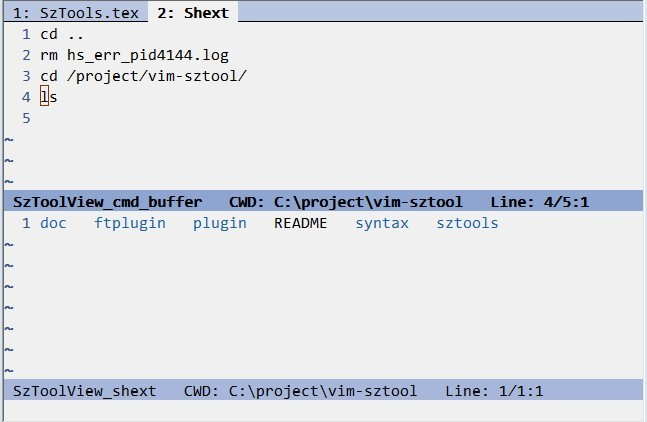
\includegraphics[scale=0.5]{shext.jpg}
  \caption{Shext截图}
  \end{figure}
  

  用\colorbox{lightgray}{:Shext}启动,启动后,会把当前buffer作为命令编辑区, 用于编辑和运行命令。 split出来的下面buffer
是命令输出区,用于显示命令的输出。在启动前,确保当前的tab页是空的。否则会把当前编辑的文件作为命令编辑区,一般这
不会是想要的情况。Shext支持内置实现的的命令和系统的命令, 内置命令优先。不支持交互式和需要用到终瑞库的命令, 如ftp,mysql,vim,mc等。 

  在命令编辑buffer, 如果输入"/",如果对应的参数是目路路径, 则在命令输出buffer会显示
对应路径的内容作为提示。 比如 
  \begin{verbatim} cd c:/ \end{verbatim}
 在"/"按下后, 会列出c:根目录的内容。(Shext默认在linux和win下都使用"/"作为目录分隔符)

  在命令编辑区, 在insert模式下输入"\$n;;", 则会把输出buffer的第n行补全到当前命令行中。
在某些条件下会比较有用。

  比如你可以先用 find --name *.java --text Apple 查找包含Apple的java文件, 在找到后,
如果想编辑其中的第5个文件, 则可以用 "edit \$5;;<cr>" 来实现。 注意这个补全是带状态的,
在\$5;;后,如果你还要编辑上一个文件,可以用<C-p>, 如果想编辑下一个文件,可以用<C-n>。


\subsection{内置命令}
     内置命令是插件自已实现的命令,大多数是linux下命令的简化版。本来这些命令直接调用系统命令会更强
大,但由于我的工作环境主要是windows,另外像ls的带色彩化输出也难以做到,所以才用python和java简化
实现了一点。ls的输出做了些定制,支持对目录和压缩文件,以及可执行文件以不同的颜色显示。具体的颜色
可以在$\tiny{\sim}$/.sztools/sztools.cfg文件中配置。

\subsubsection{改变和显示目录}

\begin{verbatim}
pwd      : 显示当前目录
cd args  : 更改当前目录,可使用bookmark和通配符。
cdlist   : 列出cd过的目录历史。
lsd      : 列出当前目录下的子目录。
\end{verbatim}

\begin{flushleft}\textbf{举例:}\end{flushleft}
\begin{mdframed}[style=SmallFrame] cd \~/.vim/plugin \end{mdframed}到home目录的.vim/plugin目录
\vspace{4mm}

\begin{mdframed}[style=SmallFrame] cd work/project \end{mdframed}其中work是定义的一个书签,并非子目录
\vspace{4mm}

\begin{mdframed}[style=SmallFrame] cd *doc \end{mdframed}如果当前目录下只有一个doc结尾的子目录,则进入该子目录
\vspace{4mm}

\begin{mdframed}[style=SmallFrame] cd ../sr*/net/s*/../../icons/ \end{mdframed}通配符和..可以结合着用
\vspace{4mm}

\begin{mdframed}[style=SmallFrame] cd - \end{mdframed}回退到cd前的目录
\vspace{4mm}

\begin{verbatim}
ls [ -l | -L ][ -t | -s | -n ] [ --help ] [args] 
列当前目录内容。 
  -l 表示长格式, 每一行列一个文件
  -t 表示按时间排序
  -s 表示按大小排序
  -n 表示按名称排序
  --help 打印ls命令的帮助信息

因为实现上的原因, 以"."开头的文件默认是不显示的, 你可以用 "ls ." 来显示所有文件
\end{verbatim}

\subsubsection{书签}
\begin{verbatim}
bmadd   : 将当前目录加到bookmarks中,能在"cd"命令中引用
bmedit  : 编辑"bookmarks"文件
bmlist  : 列出所有bookmark。
\end{verbatim}

\begin{flushleft}\textbf{举例:}\end{flushleft}
\begin{mdframed}[style=SmallFrame] bmadd \end{mdframed}
如果当前的目录为 /usr/local/tomcat,调用bmadd后,会增加一个名为tomcat的书签。
这时,随便你在哪一级目录,只要 cd tomcat 就能进到 /usr/local/tomcat。
书签以文本格式存放在$\tiny{\sim}$/.sztools/shext-bm.txt文件中。可以用bmedit命令编辑
\vspace{4mm}

\subsubsection{文件管理}
\begin{verbatim}
touch [args]       : 新建文件或者更新文件时间戳
rm  [args] [-r]    : 删除文件或目录
mkdir [args]       : 新建目录
rmdir [args]       : 删除空目录
cp  [src...][dst]  : 复制文件或目录
mv  [src...][dst]  : 移动文件或目录
echo [args]        : 打印文本消息
merge [src...][dst]: 合并多个文件
cat [arg]      : 显示文件内容
head [arg]     : 显示文件前10行
edit [args]    : 在打开新tab,并编辑文件

find [-n name][-t text] [-s size] [-p path] [--help] [args] 
查找文件。
-n name 按文件名查找
-t text 查找包含文件的文件(非正则)
-s size 按文件大小查找
命令默认在当前目录查找,可以在args中指定要查找的目录。
\end{verbatim}

\subsubsection{Locate命令}
此命令在Locate一节描述

\subsubsection{杂项}
\begin{verbatim}
help           : 打印Shext帮助信息
exit           : 退出Shext。
\end{verbatim}

\subsection{系统命令}
  Shext也支持直接执行系统命令。
  \FloatBarrier
  \begin{figure}[H]%位置选项
  \centering
  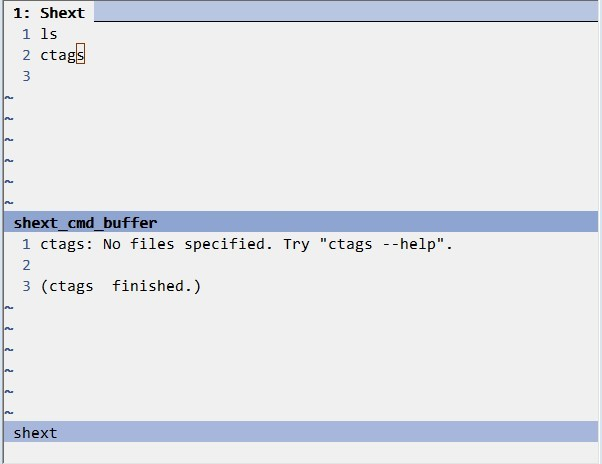
\includegraphics[scale=0.5]{shext-syscmd.jpg}
  \caption{Shext中执行系统命令截图}
  \end{figure}

  对于windows系统,可以执行"explorer ."来用资源管理器打开当前目录。

  不支持需要交互的命令,比如svn commit -m "asd"是可以的,直接svn commit却不行 ,因为后者需要输入信息

\section{Jdext}
  Jdext包含了java相关的功能,只有在Jdext启动后,本节介绍的功能才可以使用。另外在Jdext启动时,
会定义很多的map,比如\colorbox{lightgray}{<leader>go}\footnote{对于<leader>的含意,请查看vim中的帮助:help <leader>,在
默认情况下这个是指按键\textbackslash,但是我一般设置let g:mapleader = "," 。}等,如无特别说明,这些都是指normal状态
下的map。

\subsection{项目结构}
    Jdext读取的是eclipse的项目管理文件, 在项目根目中,有一个.classpath和.project文件。但是即
使没有在eclipse建项目,只要项目目录中有这两个文件,而且能正确解析的话,也是可以的。一般建
议用eclipse建立项目,包括设置类路径等。在项目建立完成后, 再在Vim中进行开发。

   对于使用maven的项目来说, 还可以直接用maven命令行建maven项目,然后用
  \begin{verbatim} mvn eclipse:eclipse \end{verbatim}
  来生成eclipse项目文件。 此种方式生成的.classpath文件,引用的jar包都是以M2\_REPO来开头的, Vim-SzTool
在默认情况下找不到这个变量相对应的路径。 需要在$\tiny{\sim}$/.sztools/vars.txt配置变量对应的路径。 格式很简单
  \begin{verbatim} M2_REPO = /usr/maven/repo \end{verbatim}

  老的maven项目,在生成.classpath文件后,需要再运行 mvn compile编译项目代码,Jdext启动时需读取
类信息,以支持代码补全功能。

   对于简单的类,如果只引用JDK自带类库的话, 也可以不用项目结构。在Jdext启动后,直接在任意目录新建Java
文件,然后就可以保存编译和调试(对于jdk自带类库的引用,也支持代码补全)。
  
   对于需要几个jar包的小工程, 也可以新建空目录后, 然后cd到空目录, 运行\colorbox{lightgray}{:InitProject}命令来初始
化项目结构。 这个命令会生成.classpath和 src,lib目录。 然后你可以拷自己的jar包到lib目录, 并自己编辑
.classpath来更新类路径。

\subsection{启动Jdext}
   有几种方式可以启动Jdext:
    \begin{enumerate}
      \item 调用:Jdext 启动, 此命令会设置很多的map,比如(保存时自动编译文件等)。 同时如果当前目录是
  在一个项目文件夹下(往上查找到.classpath文件),则Agent程序会在后台缓存类信息, 以加快补全速度。
      \item 在Shext中运行jde start命令, 功能同上。
    \end{enumerate}

\subsection{补全}
    Vim-Sztool自定义了java类型的omni\footnote{omni补全为感知上下文的补全,相当于IDE里的智能补全。vim里有多种补全方式,比如关
    键字补全。vim自带了不少omni的补全功能,比如HTML,CSS等,具体请查看vim帮助。:help new-omni-completion }的补全,编
    辑java时, 用 <ctrl-x><ctrl-o> 来进行。
    \begin{mdframed}[style=BestPracticeFrame]
      最佳实践: 安装SuperTab插件, 可以用tab键来做补全。
      Vim-Sztool会做侦测,如果已经安装SuperTab插件, 则对于java类型的文件,默认的tab补全即是omni补全。
    \end{mdframed}

    \begin{enumerate}
      \item 可以补全包名,类名,名量名和对象的成员方法和字段
      \item 方法和字段补全是 ignore case 的,且可以引用通配符,比如 aa.to*er, 可以匹配成 aa.toLower
      \item 如果是大写开头的名字,则自动在类路径中查找类名。比如即使没有import FileReader类, 打FileRe 可以补全成FileReader类 
      \item 补全类名时,不像eclipse那样能自动补上import语名。类补全完成需再\colorbox{lightgray}{<leader>ai}一下
    \end{enumerate}
    
\subsection{编译}
    保存 java 时自动编译,如果有错误,则会生成 quickfix 列表,可以用:cn,:cp命令转到前一个或后一个错误。
    对于在类路径下的资源文件,如xml或properties文件, 在保存时也会自动复制到项目的编译输出目录。
    Jdext默认的编译级别,编译encoding,这些在sztools.cfg中设置。

  \begin{figure}[htbp]%位置选项
  \centering
  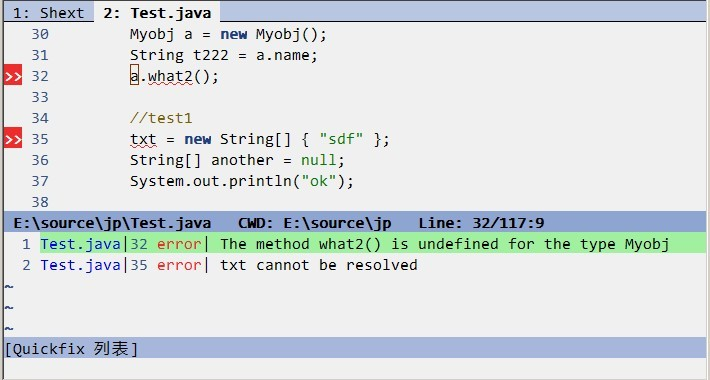
\includegraphics[scale=0.5]{compile.jpg}
  \caption{Jde保存java文件时截图}
  \end{figure}

  \begin{mdframed}[style=BestPracticeFrame]
  \begin{flushleft}
    最佳实践: 定义如下map,快速在quickfix中移动

    map <C-n> :cn<cr>\newline
    map <C-p> :cp<cr>
  \end{flushleft}
  \end{mdframed}

\subsection{运行}
    使用 \colorbox{lightgray}{:Run} 或 \colorbox{lightgray}{<leader>,} 来 运行当前的class。
注意运行的程序中不能有从终端中读取的功能,否则java程序将不能正常结束。
此功能暂不支持加arguments。如果需要测试程序参数,可以在Jdb模式启动后用 \colorbox{lightgray}{run}命令进行。

\subsection{其他功能}

\subsubsection{Import}
    对于代码中引用到的类,没在import语句中声明的,可以用 \colorbox{lightgray}{:AutoImport} 一次性生成全部import语句。 
这个命令默认的map为\colorbox{lightgray}{<leader>ai}。如果import中引用的包在源码中无引用, 则这个命令也会自动清除该import。
由于此命令基于正则,有时候会出不对的情况。

\subsubsection{生成getter,setter}
    用visual模式选中类中的属性(可以多行),\colorbox{lightgray}{<leader>gg} 来生成 getter,setter。在内部类中此命令生成的方
方位置会不对。可以自己拷到正确的位置。

\subsubsection{查看类信息}
   在编辑Java文件时,如果想快速查看某个类的信息,可以用\colorbox{lightgray}{<leader>dc}功能。这个命令会打出类的所有公共方法,
以及是否抽象方法等。(在继承实现某个类时可以用到)。

\subsubsection{跳转到类定义}
浏览Java源码时,当光标在某个方法或变量时,可以用\colorbox{lightgray}{<leader>gd} 来跳转
到定义的位置。如果光标位置的调用是一个接口的方法,而这个接口又仅有一个实现时,可以用\colorbox{lightgray}{<leader>gi}可以跳转
到接口方法实现的位置。

\subsubsection{定位本类成员}
  如果想要快速的跳转到本类的某一个方法,可以用\colorbox{lightgray}{<leader>go}。
  此功能会弹出一个类似Locate功能的界面,随着按键自动匹配成员名称。匹配到后按回车就可以跳到相
  应的成员所在的行上。如果想中止查找,可以用\colorbox{lightgray}{Esc}键。
  \begin{mdframed}[style=BestPracticeFrame]
    最佳实践: 推荐安装Tagbar插件。此插件功能类似著名的TagList,但是对面向对象语言有更好的支持。
    此插件需要ctags程序支持,程序下载后也要放在path搜索目录中。在附录中有此插件的地址。
    插件安装后最好也自定义下map如:
      nnoremap <silent> <F10> :TagbarToggle<cr>
  \end{mdframed}

\subsubsection{初始化项目结构}
使用 \colorbox{lightgray}{:InitProject} 在当前目录初始化一个 jdext 项目, 如果编辑的文件是eclipse项目下的文件,则不需要再建项目。 

\section{Jdb}
    Jdb是插件实现的java程序调试功能(跟jdk里自带的jdb程序没关系), 需要在Jdext启动后再调用。 启动后, 默认会 
    split两块buffer, 一块是jdb命令buffer, 一块是jdb命令的输出buffer。 jdb命令的buffer也是普通buffer, 除了在回车时自动执行命令(类似于shext) 

    jdb的大步部份调试功能是在jdb的buffer中用命令实现的, 有个例外是加断点。 只要启动了
    jde模式,在编辑java文件的时候,就可以用\colorbox{lightgray}{<leader>tb}来为当前行切换断点。

  \subsection{运行和附加}
    
    通过run命令运行Class, 后面为classname和参数, 如classname省略, 则运行当前编辑的Class。
    \begin{mdframed}[style=SmallFrame]
    \begin{flushleft}
    >run org.fake.test.Main --options args
    \end{flushleft}
    \end{mdframed}
    \vspace{4mm}

    attach命令运行远程连接到java程序进行调试, 要求已经运行的程序必需要jpda调试模式启动
    用此命令可以远程连接到比如tomcat之类的应用。 此命令需要一个port参数为远程调试端口号, 
    目前只能连接到本机启动的应用, 其他host暂不支持。
    \begin{mdframed}[style=SmallFrame]
    \begin{flushleft}
    >attach 8080              
    \end{flushleft}
    \end{mdframed}
    \vspace{4mm}

    disconnect命令用于断开attach上去的连接, shutdown用于中止正在调试的程序, hide用于
    隐藏jdb的窗口, exit退出调试 
    \begin{mdframed}[style=SmallFrame]
     \begin{flushleft}
    >disconnect\newline
    >shutdown\newline
    >hide\newline
    >exit                      
    \end{flushleft}
    \end{mdframed}
    \vspace{5mm}

    runtomcat命令用于从jdb从运行tomcat应用。 tomcat的配置在sztools.cfg中进行, 
    需要配置的三个属性是 tomcat\_version, tomcat\_home, tomcat\_jvmopts, 最后
    一个参数用来配置tomcat的jvm叁数。 配置中的目录,在windows下的"\textbackslash"
    需要用"\textbackslash\textbackslash"来进行。 比如
    \begin{verbatim} D:\\soft\\tomcat6 \end{verbatim}
    \begin{mdframed}[style=SmallFrame]
     \begin{flushleft}
      >runtomcat
     \end{flushleft}
    \end{mdframed}

  \subsection{检查变量}
    print(或eval)命令用于打印表达式的值。 reftype命令用于打印表达式的类型,
  inspect命令打印表达式的各个成员的值。 locals打印函数内所有本地量的值, fields
  用于打印当前对象的各个字段的值
    \begin{mdframed}[style=SmallFrame]
      \begin{flushleft}
      >print expression\newline
      >eval expression\newline
      >reftype expression\newline                      
      >inspect expression\newline                      
      >locals\newline                      
      >fields
      \end{flushleft}
    \end{mdframed}

  \subsection{跟踪}

    单步进入,单步跳过,单步跳出,恢复。 这个跟eclipse的功能差不多。 快捷键也是一样的,分
    别是<F5><F6><F7><F8>。
    \begin{mdframed}[style=SmallFrame]
      \begin{flushleft}
      >step\_into\newline
      >step\_over\newline
      >step\_return\newline
      >resume           
      \end{flushleft}
    \end{mdframed}

    

  \subsection{线程和堆栈}
  threads列出当前jvm的所有线程, thread命令用于切换当前线程(如果有线程是suspend状态的话),
  frames列出当前线程的所有调用栈。 frame命令用于切换当前的栈桢。(print,eval等命令只能打印当前栈桢的变量值)
  breakpoints列出当前jvmf所有的断点, bpa添加条件断点, setvalue改变var值
    \begin{mdframed}[style=SmallFrame]
      \begin{flushleft}
      >threads\newline
      >thread threadId\newline
      >frames\newline
      >frame n\newline
      >breakpoints\newline
      >bpa classname lineNum condition-expression\newline
      >setvalue  varname value-expression\newline
      \end{flushleft}
    \end{mdframed}

  \subsection{调试实例}
  新建测试用空目录,启动Jdext。然后新建个两个测试类,在第9行用
<leader>tb切换断点,接着启动Jdb时行调试。如下图
  \FloatBarrier
  \begin{figure}[H]%位置选项
  \centering
  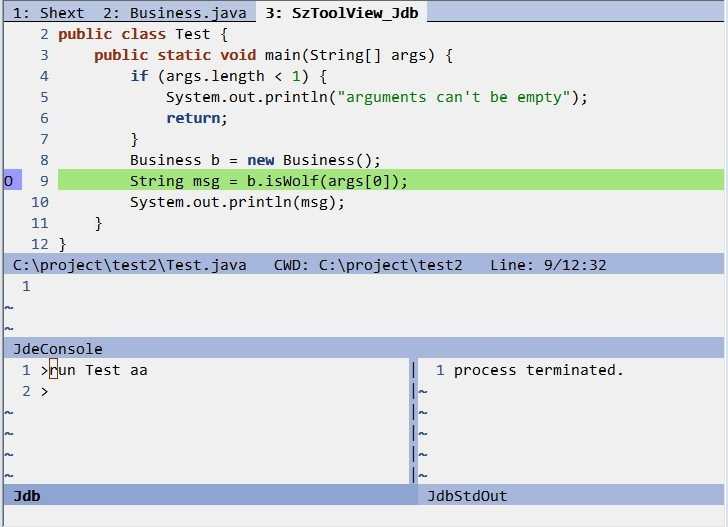
\includegraphics[scale=0.5]{jdb-run.jpg}
  \caption{Jdb运行java类}
  \end{figure}
  run命令开始后,会又新增一个"JdeConsole"的buffer以打印java程序的输出。
  此时按<F5>或在jdb命令buffer中输入step\_info, 则跳转到Business类中。
  \FloatBarrier
  \begin{figure}[H]%位置选项
  \centering
  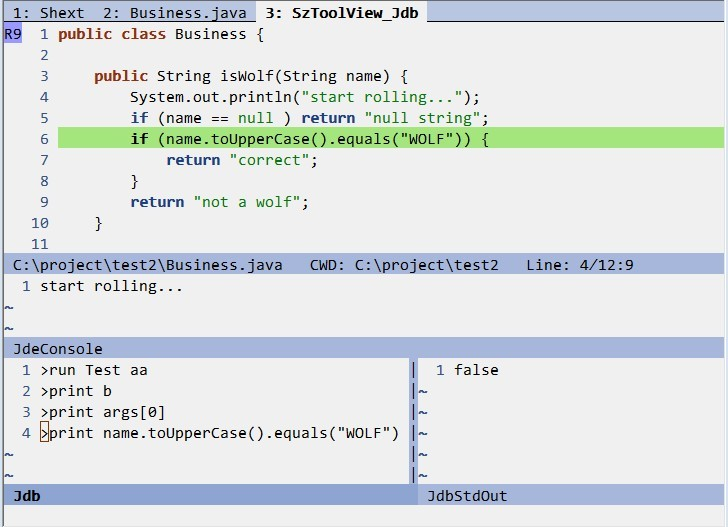
\includegraphics[scale=0.5]{jdb-print2.jpg}
  \caption{Jdb运行java类}
  \end{figure}
  执行print语句,jdb输出在"JdbStdout" buffer中显示。此时可以继续调试
或用frame切换到上一个栈帧去查看Test类中的变量的值。被调试的java类运行
结束后,会在"JdbStdout"中显示"process terminated."。调试完成后用exit命
令退出。

\section{ProjectTree}

  ProjectTree从NerdTree借鉴了相当多的代码, 基本上我写这个东西就是因为
NerdTree有些地方还难以适合做java的项目树(比如源包jar包的显示), 所以我
用python又写了一套。

  ProjectTree启动时,会从当前目录向上查找eclipse项目文件,如果找不到,就
以当前目录为树的根节点目录。如果找到项目配置.classpath文件,则会以此目录
做为树的根节点目录,同时会在根节点上增加一个叫"Referenced Libraries"的虚拟
目录节点,下面对应项目中引用的source jar包。对于没有关联源码的jar包,不会
在节点中显示。一般至少会有一个节点"src.zip",对应jdk自带的源码。
  
  \begin{mdframed}[style=BestPracticeFrame]
      最佳实践: 在用mvn eclipse:eclipse生成项目文件之前,可以配置pom文件下载关联的源码
      \begin{verbatim}
      <plugin>
        <groupId>org.apache.maven.plugins</groupId>
        <artifactId>maven-eclipse-plugin</artifactId>
        <configuration>
          <downloadSources>true</downloadSources>
          <downloadJavadocs>true</downloadJavadocs>
        </configuration>
      </plugin>
      \end{verbatim}
    \end{mdframed}

  \begin{figure}[htbp]%位置选项
  \centering
  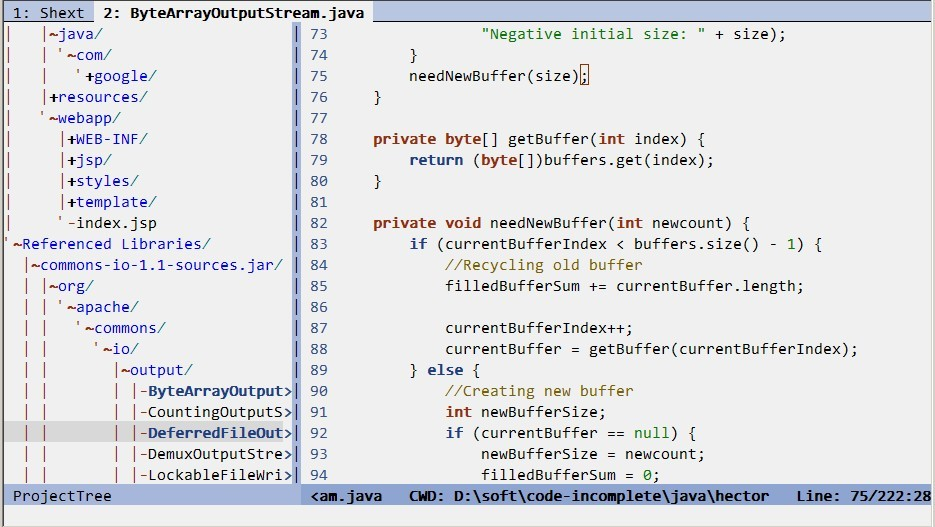
\includegraphics[scale=0.5]{tree.jpg}
  \caption{ProjectTree截图}
  \end{figure}

  ProjectTree的一些特点:
  \begin{enumerate}
    \item 按树结构显示source jar 
    \item 打开的节点显示不同的颜色,一目了然看到哪些文件在编辑
    \item 更方便的文件复制,移动,重命名功能
    \item 标记多个节点,以进行复制
    \item 按目录递归关闭正在编辑的文件
  \end{enumerate}

  \subsection{打开和关闭节点}
  在ProjectTree中打开和关闭节点是最常用的功能。 对于目录节结点来说,
打开和关闭指的是expand和collapse操作, 而对于文件节点,打开指编辑,关闭指关闭正在编辑的
文件buffer。 (在Nerdtree中对于文件节点是没有关闭操作的)
  
  正常情况下,打开文件节点后,节点会以不同的颜色显示。
  \begin{table}[H]
  \centering
      \begin{tabular}{p{40pt}p{220pt}}
        \toprule
        按键& 功能\\
        \midrule
          ?     &打印help信息\\
          <cr>  &打开选中节点\\
          o     &打开选中节点\\
          O     &递归打开选中节点\\
          t     &在新tab页中打开选中节点\\
          i     &在新window中打开选中节点\\
          go    &打开选中节点,光标停留在ProjectTree\\
          r     &刷新选中节点\\
          x     &关闭父节点\\
          s     &prompt to filter display node\\
          z     &关闭正在编辑的文件buffer, 如果当前是目录节点,则关闭目录下所有在编辑中的文件\\
          Z     &同上, 但是强行关闭文件,即使文件已改动\\
      \bottomrule
      \end{tabular}
  \end{table}

  \subsection{移动和标记}
  由于vim本身有非常多的移动功能,在ProjectTree中扩展的移动不是很多。 对于已经打开的文件,
可以用"<",">"在这些节点之前快速移动。
  \begin{table}[H]
  \centering
      \begin{tabular}{p{40pt}p{220pt}}
        \toprule
        按键& 功能\\
        \midrule
          u     &光标移动到父节点\\
          m     &标记当前节点\\
          f     &在当前节点中查找字符串\\
          >     &光标移动到下一个编辑中的文件节点\\
          <     &光标移动到上一个编辑中的文件节点\\
      \bottomrule
      \end{tabular}
  \end{table}
  另外在编辑文件的buffer, 可以用\colorbox{lightgray}{ProjectTreeFind}命令来定位左侧的
树结点。(此命令适用于左侧已经有ProjectTree打开的情况,如果还没有ProjectTree,
则可以用\colorbox{lightgray}{:ProjectTree}打开,打开时也会自动定位节点)。在我自己的vimrc中, 我
做了如下映射
  \begin{mdframed}[style=SmallFrame]
    \begin{flushleft}
      nnoremap <silent> <F9>  :ProjectTree<cr>\newline
      nnoremap <silent> <F12> :ProjectTreeFind<cr>
    \end{flushleft}
  \end{mdframed}

  \subsection{文件操作}
  以下是一些删除剪切复制的功能,注意,这些操作是同步的,即在这些
粘贴删除实际完成前, 页面将无响应。 所以不要用使用这里的功能来
操作大的文件和目录,以避免可能的vim崩溃以导致数据丢失。
  \begin{table}[H]
  \caption{删除剪切复制等}
  \centering
      \begin{tabular}{p{40pt}p{220pt}}
        \toprule
        按键& 功能\\
        \midrule
          DD    &删除选中目录或文件\\
          Dm    &删除标记的目录或文件\\
          A     &新增目录或文件(如文件名以/结尾,则为目录)\\
          ya    &复制节点路径\\
          cc    &重命名当前节点\\
          yy    &复制当前文件或目录\\
          ym    &复制标记的文件或目录\\
          dd    &剪切当前文件或目录\\
          p     &粘贴复制或剪切的文件\\
          C     &更改树的显示根目录\\
          B     &返回老的根节点\\
          U     &更改树的根节点为父目录\\
          QQ    &关闭ProjectTree\\
        \bottomrule
      \end{tabular}
  \end{table}
  ProjectTree不同于NerdTree树,它是单实例的。关闭ProjectTree树,不会删除
它的节点信息,当重新打开时,原来打开的节点或关闭的节点等都保持原来的状态。
有时候会想要完全关闭ProjectTree(比如当前目录转到其他项目文件夹之后),这时
可以先用QQ命令关闭ProjectTree,再重新打开时,就会以当前目录以树结点的根目录了。


\section{Locate}

    Locate 功能有点像command-T插件, 用来快速定位文件的。 但是不同的是,这个功能需
要先对文件夹进行索引,索引后的 文件名信息存在sqlite的数据库中。 这样无论你的当前目
录是在哪里, 都可以快速按文件名定位到已索引的目录中的文件。相当于是eclipse中的Open Resource
功能。

\subsection{索引建立删除}
  索引管理索引需要在Shext中用locatedb命令管理(建索引时需要先cd到需要索引的目录) 
  \begin{itemize}
      \item locatedb add name : 建立索引,名称为name, 索引当前文件夹的内容
      \item locatedb remove name : 删除索引
      \item locatedb refresh name : 刷新索引
      \item locatedb list : 列出已建立的索引 
  \end{itemize}

  建立索引时,并不是当前文件夹下的所有文件都会索引的。一些文件是编译输出的,或
者是临时文件的话,则默认不索引。比如.pyc文件,.class文件等默认不索引。具体哪些文件
不索引,可以通过$\tiny{\sim}$/.sztools/sztools.cfg文件中的default\_exclude\_pattern
属性值来设置。

\subsection{索引更新}
    当gvim启动后,会有一个独立的Agent进程启动,此进程会自动
监视被索引目录的文件的新建和删除,并自动更新索引。如果文件在Agent
进程未启动条件下新建和删除, 可以手动执行locatedb refresh 命令更新

   目录监视功能是系统级的,即使在vim外新增删除文件和目录也会更新索引。
想知道相关实现的可以看http://jnotify.sourceforge.net/

\subsection{调用}
   以 \colorbox{lightgray}{<leader>lw} 来启动locate模式, 启动后,底下会有一个
小的buffer用来显示匹配的文件名。 所有输入的字符都显示在command line上面,
并显示相应的匹配内容。匹配不区分大小写,并支持通配符"*"。在匹配列表出来后,可
用的功能如下
    \begin{itemize}
        \item <Esc> : 退出locate模式
        \item <CR>  : 打开(编辑)当前光标所在文件 
        \item <BS>  : 光标回退
        \item <C-j> : 光标下移
        \item <C-k> : 光标上移
        \item <C-v> : 复制剪贴板内容
        \item <C-b> : 在新buffer中打开文件
        \item <C-t> : 在新tab中打开文件
    \end{itemize}
    

\section{Dbext}

  这个是vim官方站点上的 dbext的模仿,因为之前我用原来的dbext的时候,感觉
输出不太友好(对不齐,没有表格线等,不知道新的版本有没有弄好)。然后我用python自己
实现了一个简单的。就是用pyodbc,或其他数据库驱动来执行sql,把输出结果集用表格
线排一下就得了。因为没有考虑太多,所以如果你查询大数据量的结果集,比如 
\begin{verbatim} select * from user \end{verbatim}
在user表中有几十万几上的数据的话, 很可能把vim搞死(取决于机器性能等原因)。

由于实际执行sql的是python的数据库驱动模块,所以如果想执行各种库上的SQL就要装
相应的python数据库驱动模块。一般连Ms Sql server就用pyodbc,连oracle的库就用cx\_oracle。
另外在程序中还写了mysql的驱动模块MySQLdb的支持,不过我自己用的不多,估计会有问题。

\subsection{配置}
   在使用前先确保在 $\tiny{\sim}$/.sztools 目录下的db.conf中配置了想要连接的数据库。
   配置文件格式为
    \begin{mdframed}[style=SmallFrame]
    \begin{flushleft}
    servertype="mssql",host="127.0.0.1",user="sa",password="test"\newline
    servertype="mssql",host="127.0.0.1",user="sa",password="test"
    \end{flushleft}
    \end{mdframed}
    数据库名称不需要配置,在启动Dbext后用 use databasename 来切换。servertype值
目前支持oracle,mssql,mysql,sqlite。对于sqlite,除了servertype外,另外只要一个file
属性指出sqlite库的文件位置就行了。

    请在空白的tab页上执行\colorbox{lightgray}{:Dbext},执行完后,像Shext一样会split
成两个buffer,上面一个编辑sql和执行,下面一个输出结果。在sql编辑buffer可以用 
<c-x><c-o> 来补全 , 可以补全表名,字段名... (可以用通配符) 

  \begin{figure}[htbp]%位置选项
  \centering
  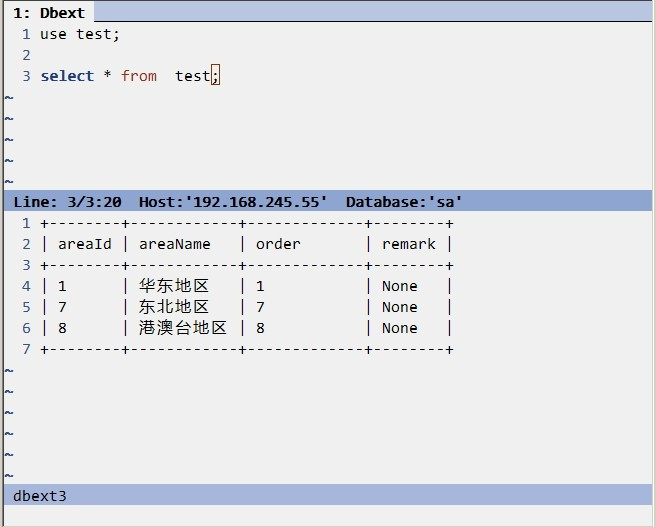
\includegraphics[scale=0.5]{dbext.jpg}
  \caption{Dbext截图}
  \end{figure}

\subsection{使用}

\subsubsection{执行查询}

    \begin{itemize} 
      \item  visual模式,选中SQL文本用 \colorbox{lightgray}{,,} 来执行,如果选中语句中有";", 默认会隔分多条来执行
      \item  normal模式和insert模式,\colorbox{lightgray}{,,}执行当前行所在的SQL语句
      \item  visual模式, \colorbox{lightgray}{,gs} 把选中文本作为单条SQL执行, 即使包含";"也不分隔
    \end{itemize} 

\subsubsection{查询元数据}

    \begin{itemize} 
    \item \colorbox{lightgray}{,ld} 用来列出所有的数据库
    \item \colorbox{lightgray}{,la} 用来列出当前数据库的所有表
    \item \colorbox{lightgray}{,dt} describe table, 列出表的字段。执行前先要visual选中表的名称
    \item \colorbox{lightgray}{,lt} 显示名称中包含当前选中文本的所有表。执行前先要visual选中文本
    \end{itemize} 

\section{杂项功能}
  \begin{itemize}
        \item <leader>te  :将选中文档用表格框起来
        \item <leader>rc  :删光java文件的注释
        \item :Example name  :split出一个buffer,显示示例文件。 示例参见安装目录下share/examples
  \end{itemize}
    

\chapter{附录}
  以下是一些你可能会想要看一下的东西:
  \newline

  \href{http://www.vim.org/scripts/script.php?script\_id=1213}{http://www.vim.org/scripts/script.php?script\_id=1213} 
  Vjde,Vim插件
  \newline

  \href{http://eclim.org/}{http://eclim.org/} Eclim, vim插件,使用eclipse作为服务端
  \newline

  \href{http://vrapper.sourceforge.net/home/}{http://vrapper.sourceforge.net/home/}
  vrapper, clipse插件,免费
  \newline

  \href{http://www.viplugin.com/}{http://www.viplugin.com/}
  viplugin,eclipse插件,收费
  \newline

  推荐的vim插件

  supertab
  \href{http://vim.sourceforge.net/scripts/script.php?script\_id=1643}
   {http://vim.sourceforge.net/scripts/script.php?script\_id=1643}

  tagbar
  \href{http://vim.sourceforge.net/scripts/script.php?script\_id=3465}
   {http://vim.sourceforge.net/scripts/script.php?script\_id=3465}

  pathogen
  \href{http://vim.sourceforge.net/scripts/script.php?script\_id=2332}
   {http://vim.sourceforge.net/scripts/script.php?script\_id=2332}

  easymotion
  \href{http://vim.sourceforge.net/scripts/script.php?script\_id=3526}
   {http://vim.sourceforge.net/scripts/script.php?script\_id=3526}

  vimwiki
  \href{http://vim.sourceforge.net/scripts/script.php?script\_id=2226}
   {http://vim.sourceforge.net/scripts/script.php?script\_id=2226}


  bufexplorer
  \href{http://vim.sourceforge.net/scripts/script.php?script\_id=42}
   {http://vim.sourceforge.net/scripts/script.php?script\_id=42}

\chapter{已知问题}


    在 windows下,默认安装的gvim73+python2.7.2 import pyodbc时会出现import error 

    默认不支持64位系统,需要替换64位的swt.jar 

    python的默认编码要和vim的默认编码保持一致,否则会出现乱码 可以分别通过 python安装目录下的
    site-packages/sitecustomize.py 和 .vimrc中的 encoding 选项来设置 

\chapter{后记}
   本文档用vim+latex写成。 感谢这两个伟大的工具

   另外特别感谢Vim草堂的各位群友,感谢他们对我提出的问题的热心解答。
   
   
\end{document}
